% !TeX root = main.tex
\section{Metodología}\label{sec-metodologia}


      \subsection{Mapeo sistemático de la literatura}\label{sub-sec-mapeo-sistematico-de-la-literatura}

        De manera general, el MSL consiste en ``una revisión amplia de estudios
        primarios en un área temática específica que tiene como objetivo
        identificar qué evidencia está disponible sobre el tema'' \cite[p. VII]{Kitchenham2007}. Particularmente, el mapeo se realizó con base
        en el proceso descrito por \textcite{Petersen2008SystematicMapping,PETERSEN20151} en cinco
        pasos como se muestra en la \Cref{fig-01}.


        \begin{figure}[htpb]
          \centering
          \caption{El proceso de mapeo sistemático.}
          \label{fig-01}
          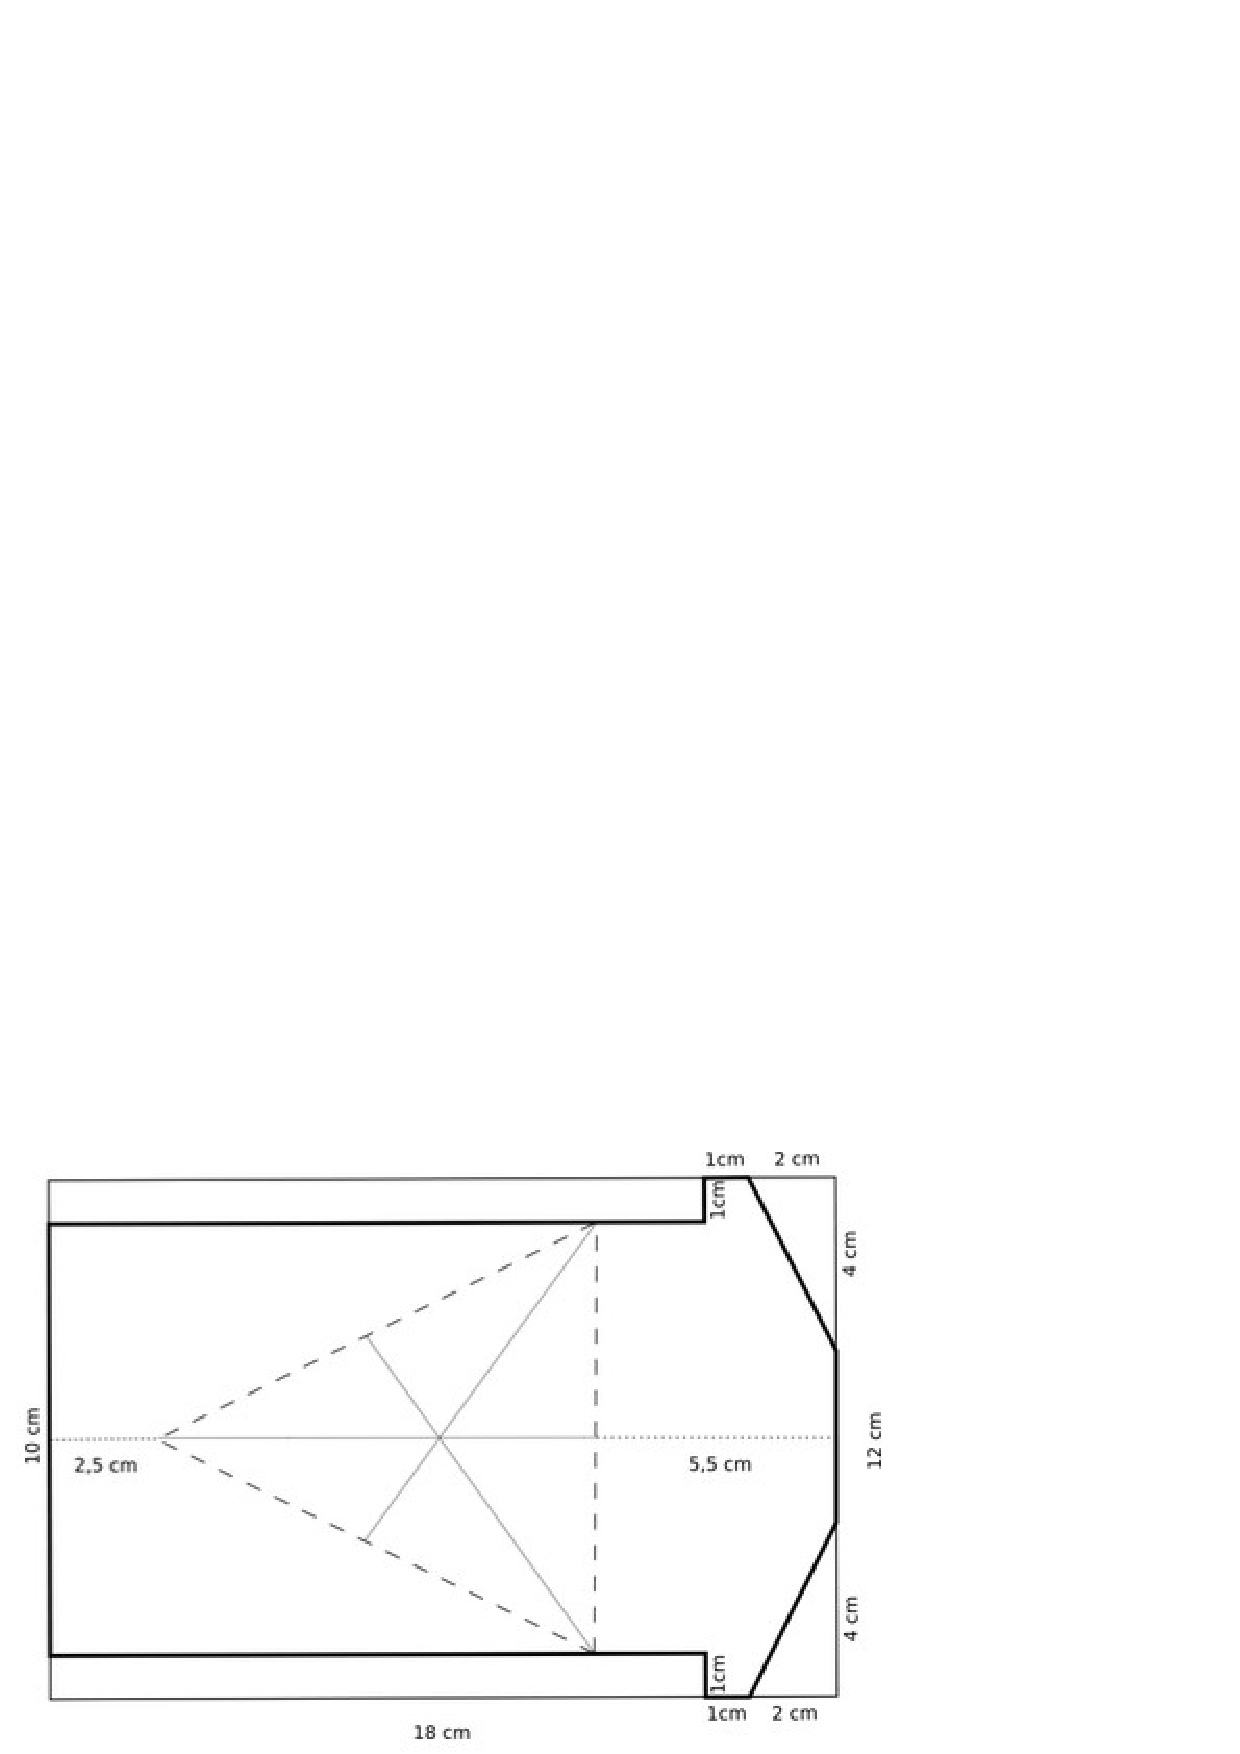
\includegraphics[width=0.75\textwidth]{figure-01.png}
          \source{Elaboración propia con base en \textcite{Petersen2008SystematicMapping}.}
        \end{figure}
        
        \subsection{Definición de preguntas y alcance de la revisión}\label{sub-sec-definicion-de-preguntas-y-alcance-de-la-revision}

        El primer paso correspondió a la estructuración de la pregunta general,
        que fungió como base para la redacción de las preguntas de investigación
        del MSL. Para su construcción se emplearon y definieron los componentes
        de Población, Intervención, Comparación, Resultados y Contexto (PICOC,
        por sus siglas en inglés) \cite{Kitchenham2007,Petticrew2006}, indicados a continuación:

        \begin{itemize}
        \item
        \textbf{Población:} institutos de educación superior, educación
        superior o educación terciaria.
        \item
        \textbf{Intervención:} proceso de transformación digital en la
        educación superior.
        \item
        \textbf{Comparación:} ninguna.
        \item
        \textbf{Resultados:} caracterización de la temática sobre
        transformación digital en la educación superior, según organismos
        internacionales.
        \item
        \textbf{Contexto:} educativo a nivel global.
        \end{itemize}

        En este sentido, la pregunta general indaga el ¿cómo ha sido la
        producción documental a nivel internacional en lo referente a la
        transformación digital en el ámbito de la educación superior, desde la
        perspectiva de organismos internacionales? Seguidamente, se derivaron
        cuatro específicas como guías del proceso del MSL y sus indicadores:

        \subsubsection{Preguntas de investigación:}\label{sub-sub-sec-preguntas-de-investigacion}

        \begin{enumerate}[label=\textbf{PI\arabic*}]

        \item ¿Qué tendencias de producción documental se observan en las
        publicaciones de organismos internacionales sobre el tema de la
        transformación digital en el ámbito de la educación superior?

        \textbf{Indicadores:} número de publicaciones por organismo
        internacional; año de publicación.

        \item ¿Cómo se caracterizan las publicaciones de organismos
        internacionales acerca de la transformación digital en el ámbito de la
        educación superior, en cuanto a país, idioma y tipo de documento?

        \textbf{Indicadores:} país de publicación; idioma de la publicación;
        tipo de recurso/material.

        \item ¿Cuáles son los contextos geográficos de estudio sobre la
        transformación digital en la educación superior en los que se han
        enfocado los organismos internacionales?

        \textbf{Indicadores:} países o zona geográfica de estudio.

        \item ¿Qué líneas temáticas sobre la transformación digital en la
        educación superior se han abordado en las publicaciones de organismos
        internacionales?

        \textbf{Indicadores:} palabras clave; resumen; objetivos; temas en
        índices.

        \end{enumerate}
    
    
 
      \subsection{Búsqueda de estudios primarios de todas las publicaciones}\label{sub-sec-busqueda-de-estudios-primarios}
    
    El segundo paso fue la localización de los estudios primarios que
    abordaran el tema de interés mediante la definición del protocolo de
    búsqueda en las bibliotecas digitales de los OI. Para ello, se revisó
    cada repositorio y se identificó que disponen de varios y distintos filtros para realizar búsquedas avanzadas (\Cref{tab-01}).

    \begin{table}[htpb]
    \centering
    \footnotesize
    \begin{threeparttable}
    \caption{Bibliotecas digitales de organismos internacionales.}
    \label{tab-01} 
    \begin{tabular}{
    >{\raggedright\arraybackslash}p{0.28\textwidth}
    >{\raggedright\arraybackslash}p{0.2\textwidth}
    >{\raggedright\arraybackslash}p{0.2\textwidth}
    >{\raggedright\arraybackslash}p{0.2\textwidth}}
        \toprule
        Organismo internacional & Nombre & \multicolumn{2}{l}{Tipos de filtros en búsquedas avanzadas} \\ 
        \midrule
        BID \url{https://publications.iadb.org/es} &
        BID Publicaciones &
            \begin{itemize}[leftmargin=*, nosep]
                \item Campo (título)
                \item Tipo de material
                \item Tema
                \item País
            \end{itemize}
         &
            \begin{itemize}[leftmargin=*, nosep]
                \item Unidad
                \item Fecha
                \item Autor
            \end{itemize}
         \\ 
    
        CEPAL \url{https://repositorio.cepal.org/home} & 
        Repositorio Digital Beta &
            Filtro básico:
            \begin{itemize}[leftmargin=*, nosep]
                \item Palabras en todo DSPACE, en una comunidad o colección
                \item Autor
                \item Subtemas ONU
                \item Fecha
                \item Tipo de recurso
                \item Formato de recurso
                \item Nivel bibliográfico
                \item Idioma
                \item País/Región
            \end{itemize}
         &
            \begin{itemize}[leftmargin=*, nosep]
                \item Serie
                \item Editorial
                \item Subtemas CEPAL
                \item Evento
                \item Símbolo ONU
                \item ODS
                \item Temas
            \end{itemize}
         \\ 
    
        OCDE \url{https://www.oecd-ilibrary.org/} &
        OECD iLibrary &
            Campos:
            \begin{itemize}[leftmargin=*, nosep]
                \item Título
                \item Autor
                \item Adscripción del autor
                \item Resumen
                \item DOI, ISBN, ISSN
            \end{itemize}
         &
            \begin{itemize}[leftmargin=*, nosep]
                \item Fecha
                \item Impresiones
                \item Idioma
                \item Tipo de contenido
                \item Tema
                \item País
            \end{itemize}
         \\ 
    
        OEI \url{https://oei.int/publicaciones} & 
        OEI Publicaciones &
            \begin{itemize}[leftmargin=*, nosep]
                \item Campo (título)
                \item Tipo de publicación
            \end{itemize}
         &
            \begin{itemize}[leftmargin=*, nosep]
                \item Fecha
                \item Áreas
                \item Oficinas
            \end{itemize}
         \\ 
        ONU/UN \url{https://digitallibrary.un.org/?ln=es} &
        Naciones Unidas Biblioteca Digital &
            \begin{itemize}[leftmargin=*, nosep]
                \item Autor
                \item Signatura
                \item Título
                \item Programa
                \item Año
                \item Resumen y notas
                \item Serie
                \item Tema
                \item Texto completo
            \end{itemize}
         &
            \begin{itemize}[leftmargin=*, nosep]
                \item Año
                \item Tipo de recurso
                \item Órgano de la ONU
            \end{itemize}
         \\ 
        Unesco \url{https://unesdoc.unesco.org/} & 
        UNESDOC Biblioteca Digital &
            \begin{itemize}[leftmargin=*, nosep]
                \item Título
                \item Autor
                \item Tema principal
                \item Tema secundario
                \item Tema geográfico
                \item Persona como tema
                \item Organización con tema
                \item Reunión como tema
                \item Obra como tema
                \item Conferencia
                \item Editor
                \item Título de la serie
                \item Código del documento
                \item ISSN
                \item ISBN
                \item DOI
            \end{itemize}
         &
            \begin{itemize}[leftmargin=*, nosep]
                \item Signatura (Biblioteca)
                \item Signatura (centros de documentos)
                \item Referencia de archivo
                \item Número de registro
                \item Palabras del registro
                \item Palabras del texto
                \item Año
                \item Tipo de material
                \item Naturaleza del contenido
                \item Fuente
                \item Licencia
                \item Idioma
                \item País
            \end{itemize}
         \\ 
	 \bottomrule
	 \end{tabular}
         \source{elaboración propia.}
	 \end{threeparttable}
	 \end{table}

    Con base en los filtros disponibles y los resultados arrojados en las
    búsquedas piloto, la cadena de búsqueda fue definida de manera
    particular en cada biblioteca digital; por lo que se emplearon e
    intercalaron en inglés y español los términos ``digital
    transformation'', ``higher education'', ``transformación digital'' y
    ``educación superior'' mediante operadores booleanos (AND/OR) (\Cref{tab-02}).
    Fue importante que en las publicaciones se mencionara el término de
    ``transformación digital'' y no solo ``digitalización'', debido a que
    son constructos que refieren a distintos niveles de alcance digital y la
    transformación es más que la digitalización \cite{grajek2020}.
    
    \begin{table}[htbp]
        \centering
        \footnotesize
        \caption{Cadenas de búsqueda en bibliotecas digitales de los organismos internacionales.}
        \label{tab-02}
        \begin{tabular}{l >{\raggedright\arraybackslash}p{0.4\textwidth}>{\raggedright\arraybackslash}p{0.4\textwidth}}
        \toprule
        \multicolumn{1}{>{\raggedright\arraybackslash}p{0.11\textwidth}}{Organismo internacional} & Cadena de búsqueda & Observación \\
        \midrule
        BID & Búsqueda avanzada en inglés: "digital transformation"
            Búsqueda avanzada en español: "transformación digital" & \begin{itemize}[leftmargin=*, nosep]
                \item ("Digital transformation" OR "transformación digital") AND ("higher
                education" OR "educación superior"), sin resultados.
                \item Búsqueda por separado de "transformación digital" y "digital
                transformation", excluyendo "educación superior" o "higher education".
                \item Búsqueda con mayores resultados: "transformación digital'' en español.
            \end{itemize} \\
        CEPAL & Búsqueda en todo DSPACE: "digital transformation" & \begin{itemize}[leftmargin=*, nosep]
                \item La cadena de búsqueda "higher education" indicó resultados lejanos a la investigación, por tanto, se excluyó en la sintaxis de exploración.
            \end{itemize} \\
            OCDE & (Title ‘Digital transformation’) (Language ‘en OR es’) AND (All Fields ‘Higher education’) & \\
            OEI & Título en español: "transformación digital" & \begin{itemize}[leftmargin=*, nosep]
                \item Solo revelaron resultados en español y sin agregar ``educación superior''.
            \end{itemize} \\
        ONU/UN & Título en inglés: "digital transformation" AND cualquier campo: "higher education" & \begin{itemize}[leftmargin=*, nosep]
                \item No se identificaron resultados en español.
                \item Se incorporaron estrategias de búsqueda por temas sin resultados.
            \end{itemize} \\
            Unesco & Búsqueda avanzada en inglés: Título: digital transformation in (Fuente: UNESCO, Idioma: español, inglés). 
            Búsqueda avanzada en español: Título: transformación digital in (Fuente: UNESCO, Idioma: español, inglés). & \begin{itemize}[leftmargin=*, nosep]
                \item Búsqueda por separado de "transformación digital'' y ``digital transformation" en ambos idiomas.
                \item Se identificaron resultados en español.
            \end{itemize} \\
            \bottomrule
        \end{tabular}
        \source{Elaboración propia.}
    \end{table}
    
    \subsection{Selección de publicaciones relevantes}\label{sub-sec-seleccion-de-publicaciones-relevantes}
    
    En el tercer paso, de acuerdo con \textcite{Kitchenham2007} y \textcite{Petersen2008SystematicMapping,PETERSEN20151}, los criterios de selección son
    utilizados para distinguir los estudios pertinentes que contribuyen a
    abordar las preguntas de investigación. Estos criterios se establecen en
    el protocolo de la revisión sistemática y se ajustan durante el proceso
    de búsqueda para minimizar el sesgo y garantizar una clasificación
    adecuada de la información.
    
    En la \Cref{tab-03} se especifican los criterios de inclusión y exclusión que
    se ajustaron durante el proceso de búsqueda realizado del 15 al 19 de
    octubre de 2023.
    
    \begin{table}[htpb]
        \centering
        \small
        \caption{criterios de inclusión y exclusión en las búsquedas.}
        \label{tab-03}
        \begin{tabular}{
        >{\raggedright\arraybackslash}p{0.11\textwidth}
        >{\raggedright\arraybackslash}p{0.4\textwidth}
        >{\raggedright\arraybackslash}p{0.4\textwidth}
        }
            \toprule
            Criterios & Inclusión & Exclusión \\
            \midrule
            Tema & Transformación digital/digital transformation
            Educación superior/higher education &
            No referidos a la transformación digital y al ámbito de la educación superior o nivel terciario \\
            Tipo de publicación & Informes, agendas, reportes, proyectos, políticas e iniciativas & \\
            Tipo de material & Libro, capítulo de libro, artículo, informe técnico, programa, reunión & Posters, resúmenes de otros documentos en extenso y traducciones de un mismo documento seleccionado \\
            Fecha & Sin delimitar & \\
            Idioma & Inglés y español & \\
            Tipo de acceso & Acesso abierto & Acceso cerrado o restringido \\
            Nivel educativo & Educación superior o terciaria & Educación básica y secundaria \\
            Unidad/Área & División de educación & Distintas a educación\\
            \bottomrule
        \end{tabular}
        \source{Elaboración propia.}
    \end{table}
    
    Particularmente, la búsqueda inicial del 19 de octubre de 2023 en ECLAC
    (Economic Commission for Latin America and the Caribbean) Library de la
    CEPAL se redirigió al Repositorio Digital beta de dicho organismo,
    debido a que este portal contiene publicaciones propias de la Comisión y
    de otros OI. Por consiguiente, se realizó otra pesquisa el 12 de enero
    de 2024, restringida entre 1950 a 2023; en coincidencia con el periodo
    de resultados de la indagación en las otras bibliotecas digitales del
    BID, la OCDE, la OEI, la ONU/UN y la Unesco.
    
    Durante la etapa de selección de documentos, se emplearon criterios de
    exclusión que implicaron revisar los títulos, resúmenes, índices de
    contenido y objetivos. Se excluyeron aquellos que estaban duplicados, de
    acceso restringido, correspondían a traducciones y resúmenes que no
    abordaban directamente el tema de la transformación digital ---solo la
    mencionaban--- o no estaban centrados en el ámbito de la educación
    superior. Como primer resultado, se descartaron 233 publicaciones del
    total de 356. Identificándose 23 documentos relevantes para la
    investigación (\Cref{tab-04}).

    %Tabela parece devidamente formatada, mas ultrapassou limite da página. Soluções: 1) ajustar o tamanho da tabela (solução pouco viável); 3) rotacionar a tabela; 4) aumentar o limite de tamanho da página; 5) diminuir tamanho da tabela/da fonte.
    
    \begin{table}[htpb]
    \centering
    \small
    \begin{threeparttable}
    \caption{Proceso de búsqueda y selección de documentos.}
    \label{tab-04}
    \begin{tabular}{
    >{\raggedright\arraybackslash}p{0.25\textwidth}
    *{7}{l}
    }
    \toprule
    Procedimento & \multicolumn{6}{c}{Organismo internacional} & Total \\
            & BID & CEPAL & OCDE & OEI & ONU/ UN & Unesco & \\
    \midrule
            Búsqueda inicial & 95 & 173 & 62 & 5 & 5 & 16 & 356 \\
            Refinamiento por unidad, división, área o subtema en educación
            & 13 & 16\tnote{a} & 10 & 3 & 3 & 15 & 60 \\
            Acceso limitado o de suscripción & 13 & 16 & 5 & 3 & 3 & 15 &
            55 \\
            Eliminación de duplicados y/o traducciones & 11 & 16 & 5 & 3 &
            3 & 13 & 51 \\
            Eliminación de documentos por contener una sección o parte de otro documento seleccionado & 11 & 16\tnote{b} & 4 & 3 & 3 & 10 &
            47 \\
            Eliminación de documentos no enfocados a la transformación digital & 11 & 10 & 4 & 3 & 2 & 8 & 38 \\
            Eliminación de documentos no enfocados al nivel superior o educación terciaria & 6 & 6 & 4 & 2 & 1 & 5 & 24 \\
            Selección de publicaciones relevantes & 5 & 6
            & 4 & 2 & 1 & 5 & 23 \\
            \bottomrule
        \end{tabular}
        \source{Elaboración propia.}
        \begin{tablenotes}
        \small {
        \item[a]{Durante el proceso de refinamiento por subtemas en educación en la biblioteca digital de la CEPAL, se agregó un documento relevante que resultó al activar el filtro "Subtemas ONU" y que no se reflejaba al activar educación en "Subtemas CEPAL".}
        \item[b]{Se sustituyó un documento que contenía una parte de otro documento en extenso por la publicación de referencia original y en extenso.}
        }
        \end{tablenotes}
        \end{threeparttable}
    \end{table}

    
    \subsection{Elaboración del esquema de clasificación}\label{sub-sec-elaboracion-del-esquema-de-clasificacion}
    
    
    Después, se procedió a la elaboración de un esquema de clasificación de
    las publicaciones relevantes, con base en el procedimiento definido por
    \textcite{Petersen2008SystematicMapping}. Específicamente, este refiere a una forma
    de definir un conjunto de categorías que permitan ubicar y agrupar los
    tipos de contenidos tratados en las distintas publicaciones y su
    contribución al campo de estudio, con el cual se pueden identificar
    líneas para investigaciones futuras.
    
    Para la clasificación, primero se leyeron los resúmenes, con el cual se
    identificaron los elementos y las palabras clave que reflejaban la
    contribución del documento, en el siguiente paso. Cuando la publicación
    no contenía resumen, palabras clave o refería a información imprecisa
    sobre el tema de interés, se revisaron el índice, el prólogo, la
    introducción y/o las conclusiones. Como siguiente paso, y con el interés
    de desarrollar un mayor nivel de comprensión sobre estos aspectos clave,
    se generaron las categorías y, seguidamente, se agruparon las
    publicaciones seleccionadas en dichas clasificaciones. De acuerdo con
    \textcite[p.~5]{Petersen2008SystematicMapping}, ``el esquema de clasificación evoluciona
    mientras se realiza la extracción de datos, como agregar nuevas
    categorías o fusionar y dividir categorías existentes''. En suma,
    se crearon tres categorías principales y una subcategoría (\Cref{tab-05}).:
    
    \begin{longtable}{
    >{\raggedright\arraybackslash}p{0.225\textwidth}
    >{\raggedright\arraybackslash}p{0.125\textwidth} 
    >{\raggedright\arraybackslash}p{0.65\textwidth}}
    	\caption{Esquema de clasificación de las publicaciones.}
    	\label{tab-05}\\
        \toprule
        Categorías & Aspecto & Descripción \\
        \midrule
        \endhead
        \multirow{3}{=}{Perspectiva temática
            (con base en \textcite{bikse2021} y \textcite{benavides2020-castro})} & Tecnológica & La tecnología funge como apoyo al
        personal, la enseñanza, la innovación, la gestión, el acceso, la
        apertura al mercado, el desarrollo, la sociedad y la investigación. Se
        incluyen computadoras, \emph{software}, redes sociales, identificación
        por radiofrecuencia (RFID), sistemas de gestión del aprendizaje (LMS),
        big data, tecnología educativa digital, repositorios, Internet de las
        cosas (IoT), arquitectura de datos, \emph{blockchain}, computación en la
        nube, inteligencia artificial (IA), ecosistema de digitalización,
        servicios móviles, realidad virtual y aprendizaje automático. \\
        & Organiza-cional & Las tecnologías están relacionadas con las funciones
        y metas que la institución busca abordar; específicamente con la mejora
        de la gestión, los planes de estudio, la docencia, la investigación, los
        procesos de negocios y el marketing digital. Destacan recursos
        tecnológicos digitales como computadoras y \emph{software}, sistemas de
        gestión laboral y marcos comerciales. \\
        & Social & El objetivo es desarrollar competencias laborales y favorecer
        el crecimiento y bienestar de los involucrados, así como facilitar el
        acceso a la educación. Comprende al gobierno, la industria, la comunidad
        interna y externa de la institución. Incluyen las tecnologías de la
        información y comunicación (TIC), las plataformas digitales y de redes
        sociales, los sistemas de gestión del aprendizaje y los sistema de
        información. \\
        
        \multirow{9}{*}{\begin{minipage}{\textwidth-0.125\textwidth-0.65\textwidth} Tipo de aporte\end{minipage}} & Modelo & Modelo educativo con
        sus contenidos e implementación. \\
        & Método & Se presenta en el texto o como anexo el proceso metodológico
        del estudio. \\
        & Instrumento & Incorpora el instrumento utilizado en la recolección de
        información para el estudio: cuestionario, guion de entrevista, rúbrica,
        otro. \\
        & Programa/ iniciativa & Se presentan iniciativas de programas o
        proyectos educativos. \\
        & Enfoque & Se exterioriza una nueva perspectiva de análisis de la
        transformación digital. \\
        & Guía/ Marco de indicadores & Marco de seguimiento e indicadores para medir
        aspectos de la transformación digital en los sistemas de educación. \\
        
        %Quebra de linha automática não funcionou. Talvez por causa de um pacote de idiomas e quebra de linhas automática?
        & \multirow{3}{*}{\begin{minipage}{0.125\textwidth} Recomendaciones \end{minipage}} & Se comunican lineamientos a modo de recomendación
        para la mejora, implementación o seguimiento de procesos de la
        transformación digital. \\
        & & Se comunican lineamientos a modo de recomendación para la mejora, implementación o seguimiento de procesos de la transformación digital. \\
        && Subcategoría: Tipo de recomendaciones \\
        && \begin{enumerate}
            \def\labelenumi{\alph{enumi})}
            \item Política pública y/o educativa.
        \end{enumerate} \\
        && \begin{enumerate}
            \def\labelenumi{\alph{enumi})}
            \setcounter{enumi}{1}
            \item Acciones/prácticas/direcciones en general.
        \end{enumerate} \\
        
        \multirow{6}{*}{\begin{minipage}{\textwidth-0.125\textwidth-0.65\textwidth}Enfoque de investigación  
            (Con base en \textcite{Wieringa2006}) \end{minipage}} & Evaluación & Se fundamenta en un problema real o la
        aplicación de una técnica específica a través de métodos empíricos como
        estudios de caso, investigaciones de campo, experimentos entre otros. \\
        & Propuesta de solución & Se plantea una metodología de resolución que
        argumenta su importancia ---aún sin ser validada por completo---, que
        representa una mejora sustancial respecto a las técnicas ya
        existentes. \\
        & Validación & Se exploran las características de una posible solución
        no aplicada en la realidad, que podría haber sido sugerida por el autor
        mismo o por alguien más. El estudio conlleva un enfoque de investigación
        metodológicamente riguroso. \\
        & Filosófica & Presentan una perspectiva innovadora, un enfoque
        conceptual nuevo. \\
        & De opinión & Contienen la opinión del autor sobre algo, cómo debemos
        hacerlo y los puntos de vista, entre otros. \\
        & Experiencia & El énfasis corresponde al aspecto "qué" en lugar del
        "por qué". La experiencia puede ser anecdótica, o relacionarse con uno o
        más proyectos, sobre la vivencia personal del autor. Requiere incluir
        una lista de lecciones aprendidas por el autor, derivadas de su
        experiencia. \\
        \bottomrule
        \source{elaboración propia} \\
    \end{longtable}
    
    \subsection{Extracción y mapeo de datos}\label{sub-sec-extraccion-y-mapeo-de-datos}    
    
    En este último paso, se integraron dos grupos de indicadores en Excel
    para recopilar la información que permitiera dar respuesta a las
    preguntas de investigación planteadas. El primero, refirió a información
    básica, tales como organismo internacional, año, país e idioma de
    publicación y tipo de recurso o material. En el segundo grupo se
    incluyeron elementos de palabras clave, resumen, objetivo, contexto
    (país o zona geográfica de estudio), temas en índices, conclusiones y
    recomendaciones.
    
    
   
